\documentclass[11pt,]{article}
\usepackage[left=1in,top=1in,right=1in,bottom=1in]{geometry}
\newcommand*{\authorfont}{\fontfamily{phv}\selectfont}
\usepackage[]{mathpazo}
\usepackage{amsmath}
\usepackage{graphicx}
\usepackage{float}
  \usepackage[T1]{fontenc}
  \usepackage[utf8]{inputenc}



\usepackage{abstract}
\renewcommand{\abstractname}{}    % clear the title
\renewcommand{\absnamepos}{empty} % originally center

\renewenvironment{abstract}
 {{%
    \setlength{\leftmargin}{0mm}
    \setlength{\rightmargin}{\leftmargin}%
  }%
  \relax}
 {\endlist}

\makeatletter
\def\@maketitle{%
  \newpage
%  \null
%  \vskip 2em%
%  \begin{center}%
  \let \footnote \thanks
    {\fontsize{18}{20}\selectfont\raggedright  \setlength{\parindent}{0pt} \@title \par}%
}
%\fi
\makeatother



\usepackage{longtable,booktabs}


\title{Estimated parameters for Schistosomiasis in Sub-saharan Africa  }





\author{}

\setcounter{secnumdepth}{0}
\date{}

\usepackage{titlesec}

\titleformat*{\section}{\normalsize\bfseries}
\titleformat*{\subsection}{\normalsize\bfseries}
\titleformat*{\subsubsection}{\normalsize\itshape}
\titleformat*{\paragraph}{\normalsize\itshape}
\titleformat*{\subparagraph}{\normalsize\itshape}


\usepackage{natbib}
\bibliographystyle{apalike}
\usepackage[strings]{underscore} % protect underscores in most circumstances



\newtheorem{hypothesis}{Hypothesis}
\usepackage{setspace}

\makeatletter
\@ifpackageloaded{hyperref}{}{%
\ifxetex
  \PassOptionsToPackage{hyphens}{url}\usepackage[setpagesize=false, % page size defined by xetex
              unicode=false, % unicode breaks when used with xetex
              xetex]{hyperref}
\else
  \PassOptionsToPackage{hyphens}{url}\usepackage[unicode=true]{hyperref}
\fi
}

\@ifpackageloaded{color}{
    \PassOptionsToPackage{usenames,dvipsnames}{color}
}{%
    \usepackage[usenames,dvipsnames]{color}
}
\makeatother
\hypersetup{breaklinks=true,
            bookmarks=true,
            pdfauthor={},
             pdfkeywords = {},  
            pdftitle={Estimated parameters for Schistosomiasis in Sub-saharan Africa},
            colorlinks=true,
            citecolor=cyan,
            urlcolor=blue,
            linkcolor=magenta,
            pdfborder={0 0 0}}
\urlstyle{same}  % don't use monospace font for urls

% set default figure placement to htbp
\makeatletter
\def\fps@figure{htbp}
\makeatother

\usepackage[english]{babel}
\usepackage{booktabs}
\usepackage{longtable}
\usepackage{array}
\usepackage{multirow}
\usepackage[table]{xcolor}
\usepackage{wrapfig}
\usepackage{float}
\usepackage{colortbl}
\usepackage{pdflscape}
\usepackage{tabu}
\usepackage{threeparttable}
\usepackage{threeparttablex}
\usepackage[normalem]{ulem}
\usepackage{makecell}


% add tightlist ----------
\providecommand{\tightlist}{%
\setlength{\itemsep}{3pt}\setlength{\parskip}{0pt}}

\begin{document}
	
% \pagenumbering{arabic}% resets `page` counter to 1 
%
% \maketitle

{% \usefont{T1}{pnc}{m}{n}
\setlength{\parindent}{0pt}
\thispagestyle{plain}
{\fontsize{18}{20}\selectfont\raggedright 
\maketitle  % title \par  

}

{
   \vskip 13.5pt\relax \normalsize\fontsize{11}{12} 
 

}

}






\vskip 6.5pt


\noindent  \hypertarget{data-processing}{%
\section{Data processing}\label{data-processing}}

ESPEN data was checked for the presence of duplicated locations. Only
locations replicated over time where found and, for each of these
entries, the most recent survey was retained. All the countries with
less than 50 surveys were excluded from modelling.

\hypertarget{modelling-framework}{%
\section{Modelling framework}\label{modelling-framework}}

We fit a binomial geostatistical model to Schistosomiasis data for each
country both for Haematobium and for Mansoni. The number of individuals,
\(y_i\), tested positive for Schistosomiasis out of the number of people
examined \(n_i\) at each location \(x_i\) can be considered as the
realisation of a Binomial random variable
\(Y_i \sim \text{Binom}(n_i, p(x_i))\), with \(p(x_i)\) modelled as:
\[\log\left\{\frac{p(x_i)}{1 - p(x_i)}\right\}=\mu+S(x_i) + Z_i\] where
\(S(x)\) is a zero mean Gaussian process with variance \(\sigma^2\) and
an exponential correlation function given by
\(\rho(u;\phi)=\exp\{-u/\phi\}\) where \(\phi > 0\) is a scale parameter
that controls the extent of the spatial correlation and \(u\) is the
distance between two sampling locations. Moreover, \(Z_i\) is a set of
independent zero-mean Gaussian variables with mean \(0\) and variance
\(\tau^2\).

\hypertarget{results}{%
\section{Results}\label{results}}

\autoref{tab:haema} and \autoref{tab:mansoni} report the estimated
parameters obtained by fitting a binomial geostatistical model to
Haematobium and Mansoni pre-intervention data respectively. In
\autoref{fig:plots} we compare the distribution of the estimated model
parameteres for the two species.

\begin{longtable}[]{@{}lccccl@{}}
\caption{\label{tab:haema} Monte Carlo maximum likelihood estimates for
the model fitted to Haematobium data.}\tabularnewline
\toprule
Country & n & \(\hat{\mu}\) & \(\hat{\sigma}^2\) & \(\hat{\phi}\) &
\(\hat{\tau}^2\)\tabularnewline
\midrule
\endfirsthead
\toprule
Country & n & \(\hat{\mu}\) & \(\hat{\sigma}^2\) & \(\hat{\phi}\) &
\(\hat{\tau}^2\)\tabularnewline
\midrule
\endhead
Benin & 286 & 0.126 & 2.120 & 17.919 & 1.395\tabularnewline
Burkina Faso & 192 & 0.068 & 1.593 & 29.094 & 2.679\tabularnewline
Chad & 178 & 0.171 & 2.629 & 84.547 & 0.796\tabularnewline
Congo (Kinshasa) & 226 & 0.039 & 1.842 & 118.435 & 1.468\tabularnewline
Cote D'ivoire & 433 & 0.008 & 4.118 & 52.093 & 1.856\tabularnewline
Gabon & 110 & 0.027 & 1.163 & 26.165 & 0.000\tabularnewline
Ghana & 146 & 0.092 & 3.389 & 147.868 & 2.186\tabularnewline
Kenya & 170 & 0.057 & 5.001 & 51.530 & 1.216\tabularnewline
Liberia & 1028 & 0.013 & 6.582 & 62.273 & 0.816\tabularnewline
Madagascar & 150 & 0.162 & 7.255 & 83.054 & 0.618\tabularnewline
Malawi & 641 & 0.049 & 1.082 & 72.034 & 1.334\tabularnewline
Mali & 165 & 0.181 & 2.703 & 101.656 & 2.532\tabularnewline
Mauritania & 52 & 0.062 & 3.309 & 211.459 & 0.758\tabularnewline
Namibia & 256 & 0.002 & 14.432 & 853.474 & 2.083\tabularnewline
Niger & 685 & 0.042 & 1.490 & 86.200 & 3.534\tabularnewline
Nigeria & 1584 & 0.062 & 2.502 & 72.221 & 1.569\tabularnewline
Rwanda & 94 & 0.007 & 0.008 & 4.078 & 0.002\tabularnewline
Senegal & 209 & 0.062 & 5.564 & 85.502 & 2.863\tabularnewline
South Sudan & 162 & 0.004 & 2.799 & 17.195 & 0.040\tabularnewline
Swaziland & 202 & 0.079 & 1.024 & 29.480 & 0.370\tabularnewline
Tanzania (Mainland) & 440 & 0.077 & 6.928 & 135.691 &
0.625\tabularnewline
The Gambia & 181 & 0.119 & 0.599 & 0.901 & 0.000\tabularnewline
Togo & 741 & 0.024 & 1.964 & 36.499 & 0.671\tabularnewline
Zambia & 100 & 0.220 & 0.980 & 24.500 & 0.830\tabularnewline
\bottomrule
\end{longtable}

\begin{longtable}[]{@{}lccccl@{}}
\caption{\label{tab:mansoni} Monte Carlo maximum likelihood estimates
for the model fitted to Mansoni data.}\tabularnewline
\toprule
Country & n & \(\hat{\mu}\) & \(\hat{\sigma}^2\) & \(\hat{\phi}\) &
\(\hat{\tau}^2\)\tabularnewline
\midrule
\endfirsthead
\toprule
Country & n & \(\hat{\mu}\) & \(\hat{\sigma}^2\) & \(\hat{\phi}\) &
\(\hat{\tau}^2\)\tabularnewline
\midrule
\endhead
Burkina Faso & 129 & 0.002 & 0.000 & 14.058 & 3.019\tabularnewline
Burundi & 200 & 0.253 & 2.434 & 23.829 & 1.873\tabularnewline
Cameroon & 123 & 0.045 & 2.108 & 47.763 & 1.417\tabularnewline
Chad & 164 & 0.001 & 4.115 & 220.045 & 0.602\tabularnewline
Congo (Kinshasa) & 1071 & 0.012 & 10.207 & 197.755 &
1.556\tabularnewline
Cote D'ivoire & 400 & 0.022 & 4.424 & 100.686 & 1.498\tabularnewline
Eritrea & 131 & 0.002 & 4.356 & 49.196 & 1.016\tabularnewline
Ethiopia & 139 & 0.003 & 16.577 & 458.889 & 7.034\tabularnewline
Gabon & 96 & 0.005 & 0.093 & 4.362 & 0.078\tabularnewline
Kenya & 913 & 0.000 & 23.315 & 90.792 & 1.133\tabularnewline
Liberia & 936 & 0.067 & 4.513 & 104.628 & 0.767\tabularnewline
Madagascar & 200 & 0.006 & 8.645 & 107.561 & 1.922\tabularnewline
Malawi & 631 & 0.004 & 1.839 & 46.976 & 1.888\tabularnewline
Mali & 228 & 0.000 & 10.232 & 145.890 & 3.766\tabularnewline
Niger & 300 & 0.002 & 1.397 & 21.846 & 0.735\tabularnewline
Nigeria & 1662 & 0.003 & 3.281 & 74.988 & 0.562\tabularnewline
Rwanda & 99 & 0.005 & 5.372 & 14.013 & 0.000\tabularnewline
Senegal & 170 & 0.000 & 16.527 & 182.993 & 2.636\tabularnewline
Sierra Leone & 56 & 0.123 & 6.996 & 189.044 & 0.700\tabularnewline
South Africa & 157 & 0.003 & 0.733 & 487.697 & 0.218\tabularnewline
South Sudan & 257 & 0.020 & 4.482 & 123.826 & 0.598\tabularnewline
Swaziland & 226 & 0.005 & 0.000 & 3.338 & 0.116\tabularnewline
Tanzania (Mainland) & 526 & 0.004 & 6.853 & 85.005 &
0.760\tabularnewline
The Gambia & 105 & 0.006 & 0.124 & 1.842 & 0.000\tabularnewline
Togo & 986 & 0.004 & 5.543 & 38.810 & 0.405\tabularnewline
Uganda & 1103 & 0.034 & 5.814 & 53.140 & 1.513\tabularnewline
Zambia & 101 & 0.028 & 6.085 & 104.941 & 1.821\tabularnewline
\bottomrule
\end{longtable}

\begin{figure}

{\centering 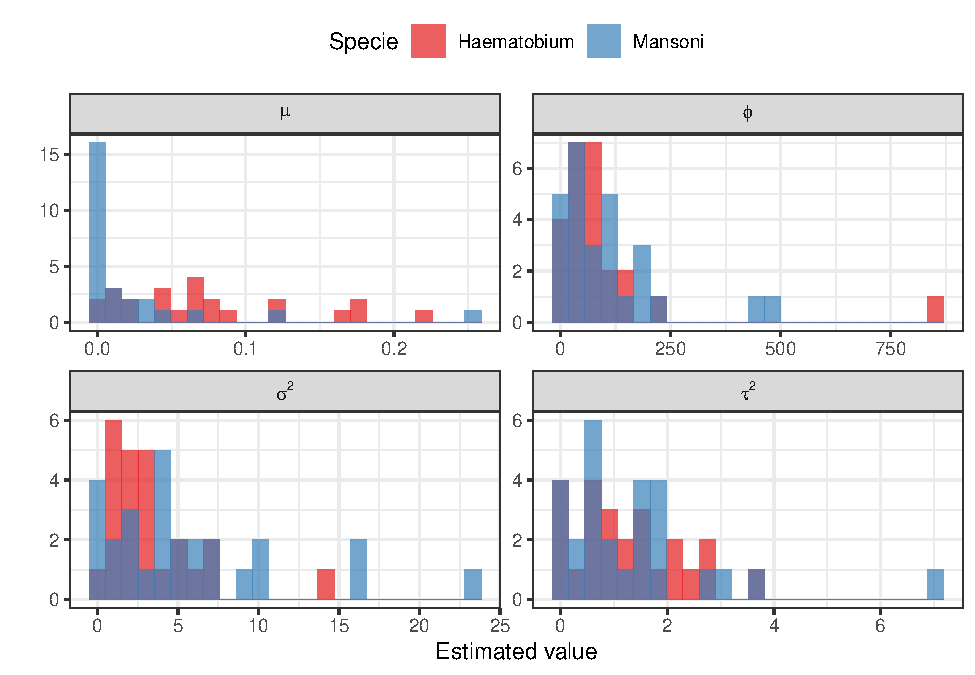
\includegraphics[width=1\linewidth]{skeleton_files/figure-latex/plots-1} 

}

\caption{Distribution of parameters estimates for both species.}\label{fig:plots}
\end{figure}




\newpage
\singlespacing 
\bibliography{biblio.bib}

\end{document}
